\chapter{Implementazione e prove sperimentali}

\section{Scenario e relative impostazioni tecnologiche}

In questa sezione sono illustrati lo scenario utilizzato e le varie misure di qualità. 
La tabella \ref{tabella_scenario} riassume le caratteristiche principali dello scenario. 
Lo scenario è statico: \textit{Illegal Dump} si basa sulla mappa di una discarica abusiva di Paternò, Italia \cite{trashout2018}.

\begin{table}[H]
    \centering
    
    \begin{tabular}{|l|c|c|c|}
    \hline
    \textbf{Scenario}              & \textbf{Area size (m x m)}                        & \textbf{No of frames}      \\ \hline
    Illegal Dump                   & 400 x 400                                         & (1)                           \\ \hline
    \end{tabular}%
    
    \caption{caratteristiche dello scenario Illegal Dump.}
    \label{tabella_scenario}
\end{table}

Per mostrare la complessità ambientale, le figure \ref{dump_map} e \ref{dump_scenario} mostrano la mappa satellitare utilizzata per \textit{Illegal Dump}, e la corrispondente immagine vettoriale iniziale rappresentata nell'ambiente di simulazione, rispettivamente. 
Qui, gli ostacoli (edifici e alberi) sono rappresentati in nero, mentre i bersagli sono rappresentati come punti rossi. 
I droni, rappresentati come triangoli viola, sono posizionati agli angoli e sono orientati verso il centro dell'area.

\begin{figure}[H] 
    \captionsetup{justification=centering, margin=2cm, font=footnotesize}
    \begin{center}
    \makebox[\textwidth]{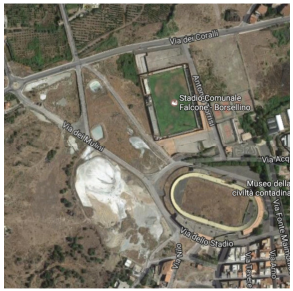
\includegraphics[width=0.3\paperwidth]{img/dump_map.png}}
    \end{center}
    \caption{Immagine satellitare dello scenario Illegal Dump.}
    \label{dump_map}
\end{figure}

\begin{figure}[H] 
    \captionsetup{justification=centering, margin=2cm, font=footnotesize}
    \begin{center}
    \makebox[\textwidth]{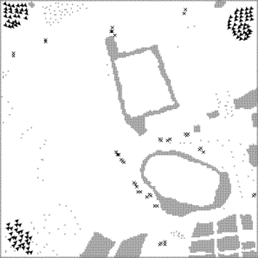
\includegraphics[width=0.3\paperwidth]{img/dump_scenario.png}}
    \end{center}
    \caption{Immagine vettoriale dello scenario Illegal Dump.}
    \label{dump_scenario}
\end{figure}

Le caratteristiche ambientali sono state prese in considerazione per le specifiche tecniche degli UAV disponibili in commercio. 
La Tabella 2 e la Tabella 3 mostrano, rispettivamente, le specifiche tecniche del drone \textit{Dji Matrice 200} \cite{matrice200}, e le apparecchiature di sensing per lo scenario di discarica illegale.
Tale tecnologia è stata selezionata sulla base delle conoscenze e delle competenze acquisite in diversi progetti che utilizzano la tecnologia UAV per il monitoraggio e la sorveglianza ambientale. 
In particolare, la tecnologia di rilevamento proposta, si basa su \cite{persechino2010aerospace} e \cite{lega2012using};

\begin{table}[H]
    \centering
    
    \begin{tabular}{|l|c|}
    \hline
    \textbf{Parameter}              & \textbf{Value}           \\ \hline
    Radius                          & $0.3 \; m$                             \\ \hline
    Max speed                       & $17 \; m/s$                             \\ \hline
    Max acceleration                & $4.4 \; m/s^{2}$                             \\ \hline
    Max angular speed               & $2.6 \; rad/s$                             \\ \hline
    Max angular acceleration        & $6.9 \; rad/s^{2}$                             \\ \hline
    battery duration                & $24-38 \; min$                             \\ \hline
    Obstacle vision distance        & $3-30 \; m$                             \\ \hline
    Obstacle vision angle           & $60\circ$                            \\ \hline
    \end{tabular}%
    
    \caption{Specifiche tecniche del modello di drone \textit{Dji Matrice 200}.}
    \label{tabella_scenario}
\end{table}

\begin{table}[H]
    \centering
    
    \begin{tabular}{|l|c|c|c|c|}
    \hline
    \textbf{Scenario}               & \begin{tabular}[c]{@{}l@{}}\textbf{Cruise speed} \\ \textbf{(m/s)}\end{tabular}                & \begin{tabular}[c]{@{}l@{}}\textbf{Sensing} \\ \textbf{technology}\end{tabular}                   & \textbf{Sensor model}                 & \begin{tabular}[c]{@{}l@{}}\textbf{Sensing} \\ \textbf{radius}\end{tabular}        \\ \hline
    Illegal Dump                    & 4                                          & \begin{tabular}[c]{@{}l@{}}Visual + \\ Thermal\end{tabular}                              & Dji Zenmuse XT2                       & 5 m                            \\ \hline    
    \end{tabular}%    
    \caption{Specifiche tecniche dell'equipaggiamento di sensing.}
    \label{tabella_scenario}
\end{table}

\section{Risultati sperimentali}

[Questo grafico è solo di test]

\begin{figure}[H] 
    \captionsetup{justification=centering, margin=2cm, font=footnotesize}
    \begin{center}
        \makebox[0.4\paperwidth]{
            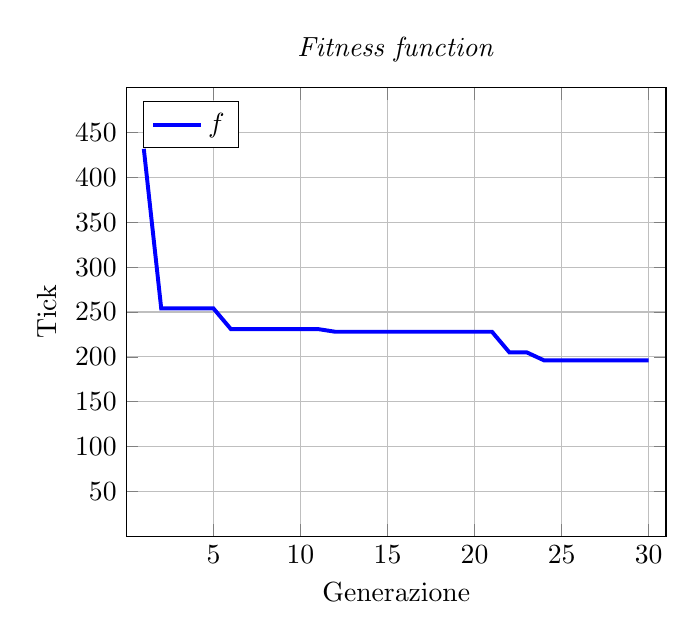
\begin{tikzpicture}
                \begin{axis}[
                    title={\textit{Fitness function}},
                    xlabel={Generazione},
                    ylabel={Tick},
                    xmin=0, xmax=31,
                    ymin=0, ymax=500,
                    xtick={5,10,15,20,25,30},
                    ytick={50, 100, 150, 200, 250, 300, 350, 400, 450},
                    legend pos=north west,
                    grid=major,
                    %ymajorgrids=true,
                    %xmajorgrids=true
                    %grid style=dashed,
                ]
                
                \addplot[
                    color=blue,
                    line width=0.5mm,
                    ]
                    coordinates {
                        (1,432.0)(2,254.0)(3,254.0)(4,254.0)(5,254.0)(6,231.0)(7,231.0)(8,231.0)(9,231.0)(10,231.0)(11,231.0)(12,228.0)(13,228.0)(14,228.0)(15,228.0)(16,228.0)(17,228.0)(18,228.0)(19,228.0)(20,228.0)(21,228.0)(22,205.0)(23,205.0)(24,196.0)(25,196.0)(26,196.0)(27,196.0)(28,196.0)(29,196.0)(30,196.0)
                    };
                    \legend{$f$}
                
                \end{axis}
            \end{tikzpicture}
        }
    \end{center}
    \caption{Andamento della funzione obiettivo al variare di generazione.}
    \label{modello3d_feromone}
\end{figure}   
    